\documentclass[a4paper, 12pt]{article}  %set doc type and font size
\usepackage{fontspec}
\usepackage[left=2cm,right=2cm,top=2.2cm,bottom=2.2cm]{geometry}

% math tools
\usepackage{amsmath}
\usepackage{amssymb}
\usepackage{amsfonts}

\usepackage[most]{tcolorbox}
\usepackage{xcolor}
\newtcolorbox{codeblock}{
  enhanced,
  breakable,
  colback=gray!5,
  colframe=black,
  boxrule=0.5pt,
  arc=2pt,
  left=6pt,
  right=6pt,
  top=6pt,
  bottom=6pt
}

\setlength{\parindent}{0pt}
% 序列標號
\usepackage{enumerate}

% 導入圖形與表格的封包
\usepackage{graphicx}
\usepackage{float}
\usepackage{booktabs}
\usepackage{tikz}
\usetikzlibrary{arrows.meta, positioning, shapes.geometric}

% set chinese
\usepackage{xeCJK}
\xeCJKsetup{AutoFakeBold=true, AutoFakeSlant=true}
\setmainfont{Times New Roman}
\setCJKmainfont{標楷體}
\XeTeXlinebreaklocale "zh"
\XeTeXlinebreakskip = 0pt plus 1pt

\title{Chapter 5　Assignment \small{Due date: June 01, 2026 (Mon)}}
\author{黃丞暘　611211106}
\date{}

\begin{document}
\maketitle % 顯示標題區塊

\section*{5.1}
\textbf{Sol.}

The EWMA is defined by
\[
E_n=\lambda X_n+(1-\lambda)E_{n-1},
\quad 0<\lambda\leq 1
\]

Expanding \(E_n\), we obtain
\[
E_n
=
\sum_{i=1}^{n}\lambda(1-\lambda)^{n-i}X_i
+
(1-\lambda)^n\mu_0
\]

Since \(n=20\) and the weight of \(X_i\) in \(E_{20}\) is
\[
w_i=\lambda(1-\lambda)^{20-i},
\quad i=1,2,\ldots,20
\]

Then we compute weights for \(\lambda=1,\ 0.5,\ 0.2,\ 0.05\) are:

\[
\begin{array}{c|c|c|c|c|c}
i & \text{Observation} & \lambda=1 & \lambda=0.5 & \lambda=0.2 & \lambda=0.05 \\ \hline
1  & X_1  & 0 & 0.000001 & 0.002882 & 0.018868\\
2  & X_2  & 0 & 0.000002 & 0.003603 & 0.019861\\
3  & X_3  & 0 & 0.000004 & 0.004504 & 0.020906\\
4  & X_4  & 0 & 0.000008 & 0.005630 & 0.022006\\
5  & X_5  & 0 & 0.000015 & 0.007037 & 0.023165\\
6  & X_6  & 0 & 0.000031 & 0.008796 & 0.024384\\
7  & X_7  & 0 & 0.000061 & 0.010995 & 0.025667\\
8  & X_8  & 0 & 0.000122 & 0.013744 & 0.027018\\
9  & X_9  & 0 & 0.000244 & 0.017180 & 0.028440\\
10 & X_{10} & 0 & 0.000488 & 0.021475 & 0.029937\\
11 & X_{11} & 0 & 0.000977 & 0.026844 & 0.031512\\
12 & X_{12} & 0 & 0.001953 & 0.033554 & 0.033171\\
13 & X_{13} & 0 & 0.003906 & 0.041943 & 0.034917\\
14 & X_{14} & 0 & 0.007813 & 0.052429 & 0.036755\\
15 & X_{15} & 0 & 0.015625 & 0.065536 & 0.038689\\
16 & X_{16} & 0 & 0.031250 & 0.081920 & 0.040725\\
17 & X_{17} & 0 & 0.062500 & 0.102400 & 0.042869\\
18 & X_{18} & 0 & 0.125000 & 0.128000 & 0.045125\\
19 & X_{19} & 0 & 0.250000 & 0.160000 & 0.047500\\
20 & X_{20} & 1 & 0.500000 & 0.200000 & 0.050000
\end{array}
\]

\begin{figure}[H]
    \centering
    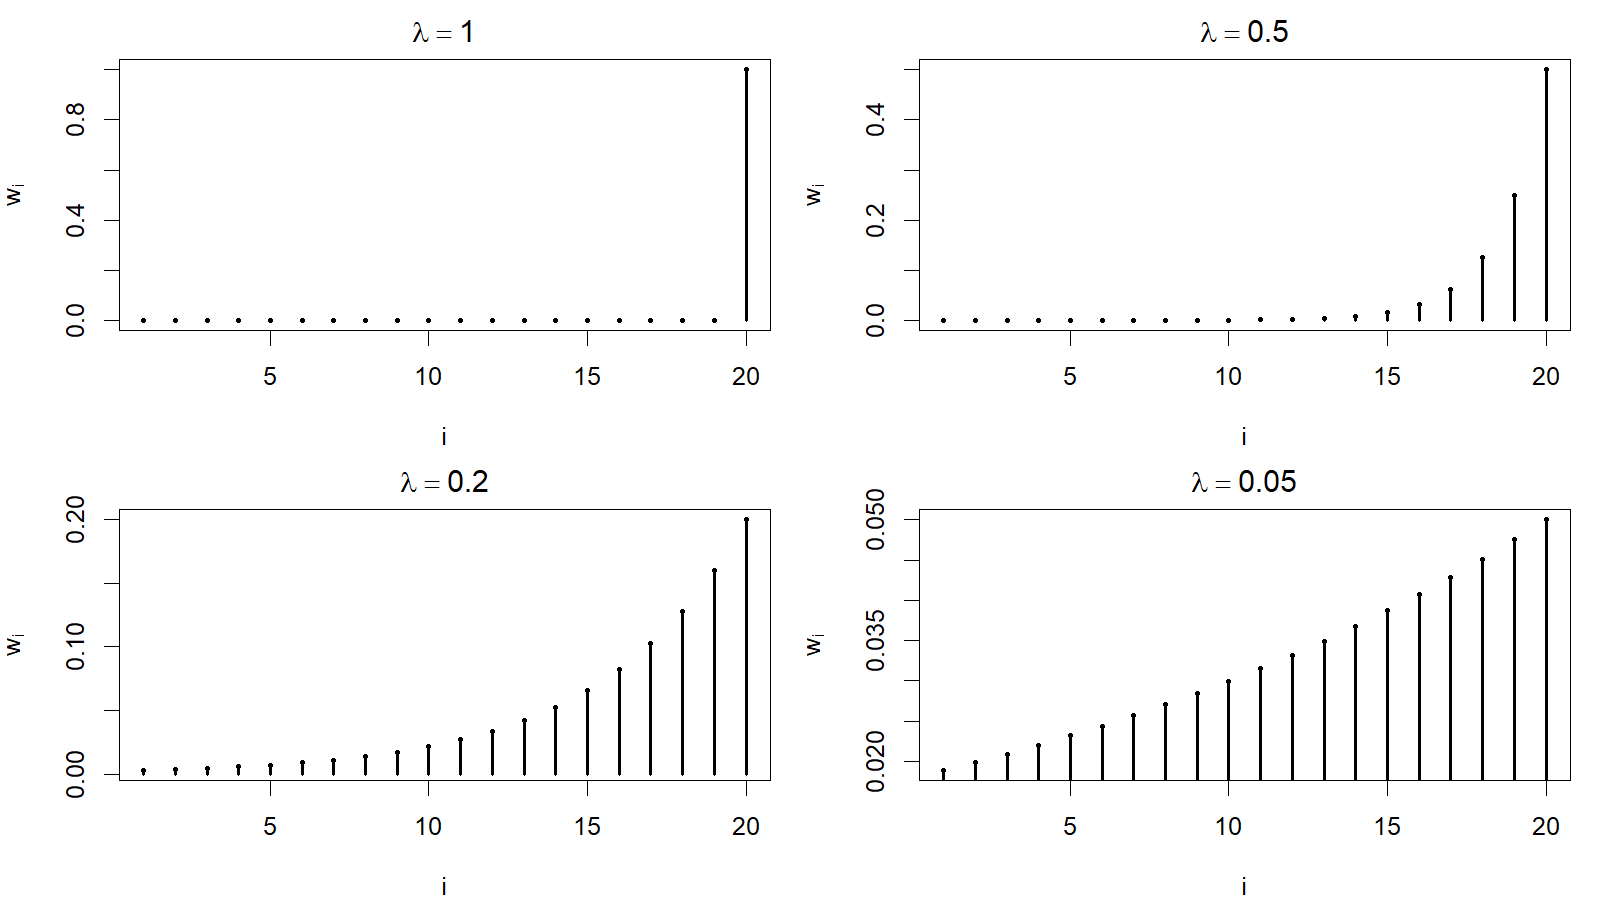
\includegraphics[width=1\textwidth]{ch5_weight_decay.png}
\end{figure}

From the figures, we can know that, when \(\lambda=1\), the EWMA statistic becomes
\[
E_n=X_n
\]
Therefore, for \(n=20\), only \(X_{20}\) receives weight 1, and all previous observations receive weight 0.

For \(0<\lambda<1\), the weight of \(X_i\) in \(E_{20}\) is
\[
w_i=\lambda(1-\lambda)^{20-i}
\]
Since \(0<1-\lambda<1\), the term \((1-\lambda)^{20-i}\) is smaller for older observations and larger for newer observations. Hence, the weights increase from \(X_1\) to \(X_{20}\).


\section*{5.4}
\textbf{Sol.}

Consider the EWMA statistic defined in (5.1),
\[
E_n=\lambda X_n+(1-\lambda)E_{n-1},
\]
and the two-sided EWMA control limits defined in (5.7)
\[
U_n
=
\mu_0+
\rho
\sqrt{
\frac{\lambda}{2-\lambda}
\left[
1-(1-\lambda)^{2n}
\right]
}\sigma,\quad
L_n
=
\mu_0-
\rho
\sqrt{
\frac{\lambda}{2-\lambda}
\left[
1-(1-\lambda)^{2n}
\right]
}\sigma
\]

We construct two-sided EWMA charts.
The first signal times are summarized as follows:
\[
\begin{array}{c|c|c|c|c}
\text{Case} & ARL_0 & \lambda & \rho & \text{First signal} \\ \hline
(i) & 200 & 0.1 & 2.454 & 17\\
(ii) & 200 & 0.5 & 2.777 & 16\\
(iii) & 500 & 0.1 & 2.814 & 18\\
(iv) & 500 & 0.5 & 3.071 & 16
\end{array}
\]

\begin{figure}[H]
    \centering
    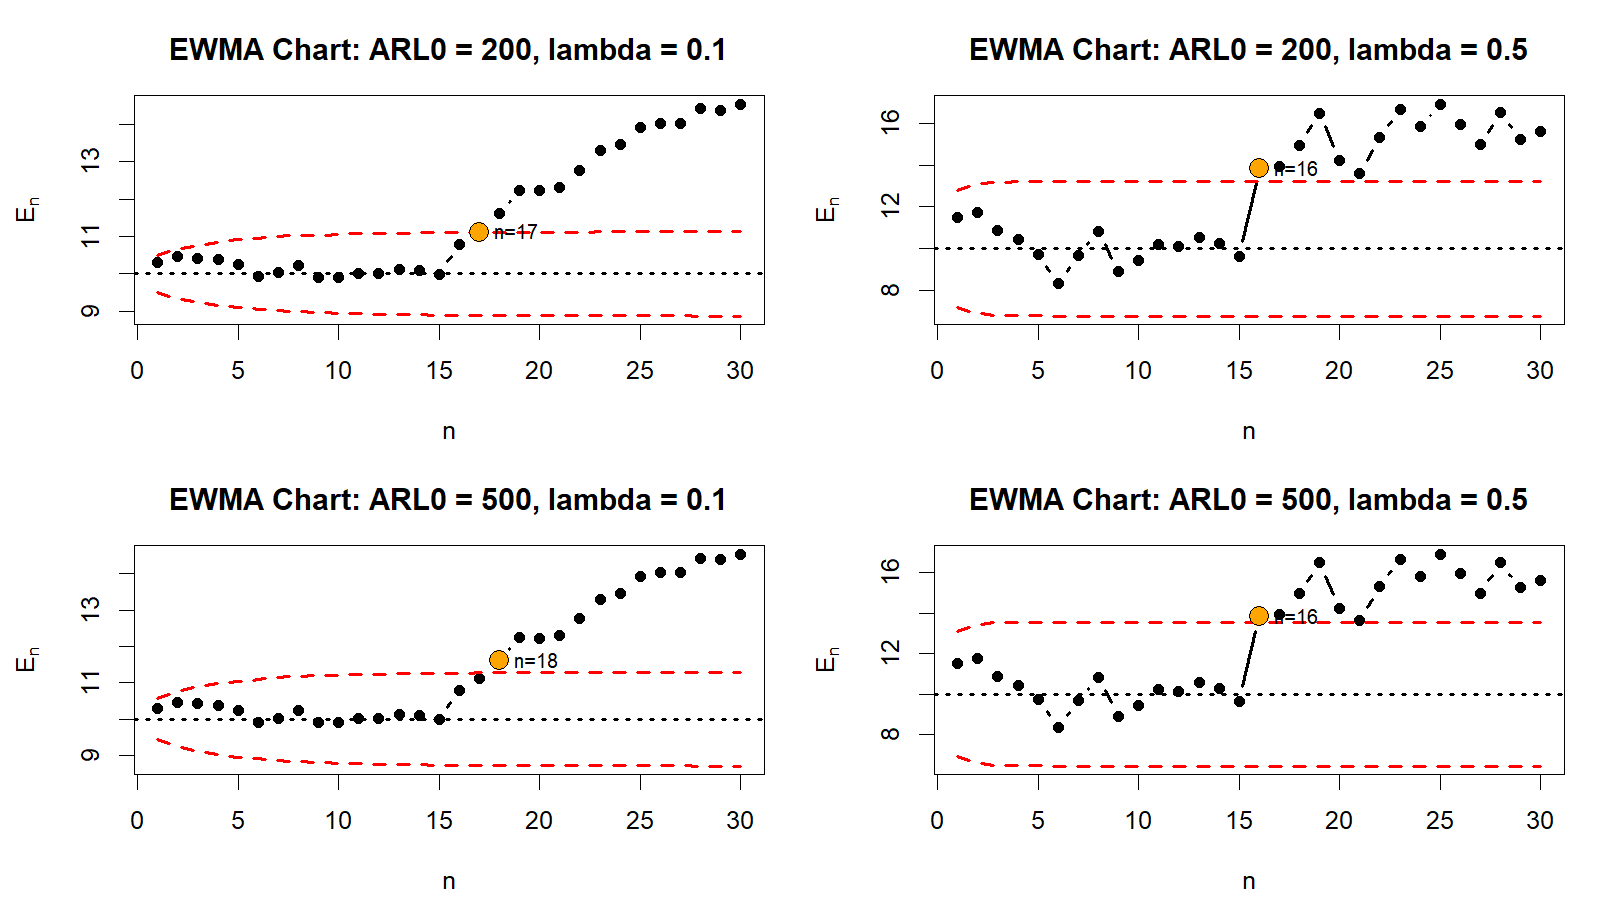
\includegraphics[width=1\textwidth]{ch5_exercise_5_4_EWMA_2x2.png}
\end{figure}

For the same \(ARL_0\), a larger \(\lambda\) gives more weight to the current observation and makes the control limits wider.
, but it also makes the EWMA statistic more sensitive to new observations. 
Therefore, the chart with \(\lambda=0.5\) signals earlier than the chart with \(\lambda=0.1\).

For the same \(\lambda\), a larger \(ARL_0\) requires a larger value of \(\rho\), which makes the control limits wider. Therefore, the chart tends to signal later.

However, when \(\lambda=0.5\), both \(ARL_0=200\) and \(ARL_0=500\) signal at \(n=16\). This happens because the upward shift is large enough that even the wider control limits for \(ARL_0=500\) are crossed at the same time.

\section*{5.6}
\textbf{Sol.}

We compute \(ARL_0\), and the results are summarized as follows:
\[
\begin{array}{c|c|c|c}
\text{Case} & \lambda & \rho & ARL_0 \\ \hline
(i) & 0.1 & 1 & 10.422\\
(ii) & 0.1 & 2 & 73.276\\
(iii) & 0.5 & 1 & 3.786\\
(iv) & 0.5 & 2 & 26.452
\end{array}
\]

From the results, for the same \(\lambda\), a larger \(\rho\) gives a larger \(ARL_0\). This is because \(\rho\) controls the width of the control limits. When \(\rho\) increases, the control limits become wider, so false alarms occur less often.

For the same \(\rho\), a larger \(\lambda\) gives a smaller \(ARL_0\).
This is mainly because \(\lambda\) controls the smoothing effect of the EWMA statistic.
When \(\lambda\) is larger, the chart gives more weight to the current observation and behaves more like a Shewhart chart. Therefore, under the IC condition, the statistic fluctuates more and is more likely to cross the control limits, leading to a smaller \(ARL_0\).

\section*{5.8}
\textbf{Sol.}

The computed \(\rho\) values are
\[
\begin{array}{c|c}
\lambda & \rho \\ \hline
0.01 & 1.500\\
0.30 & 2.713\\
0.75 & 2.802
\end{array}
\]
where each \(\rho\) is chosen so that \(ARL_0=200\).

\begin{figure}[H]
    \centering
    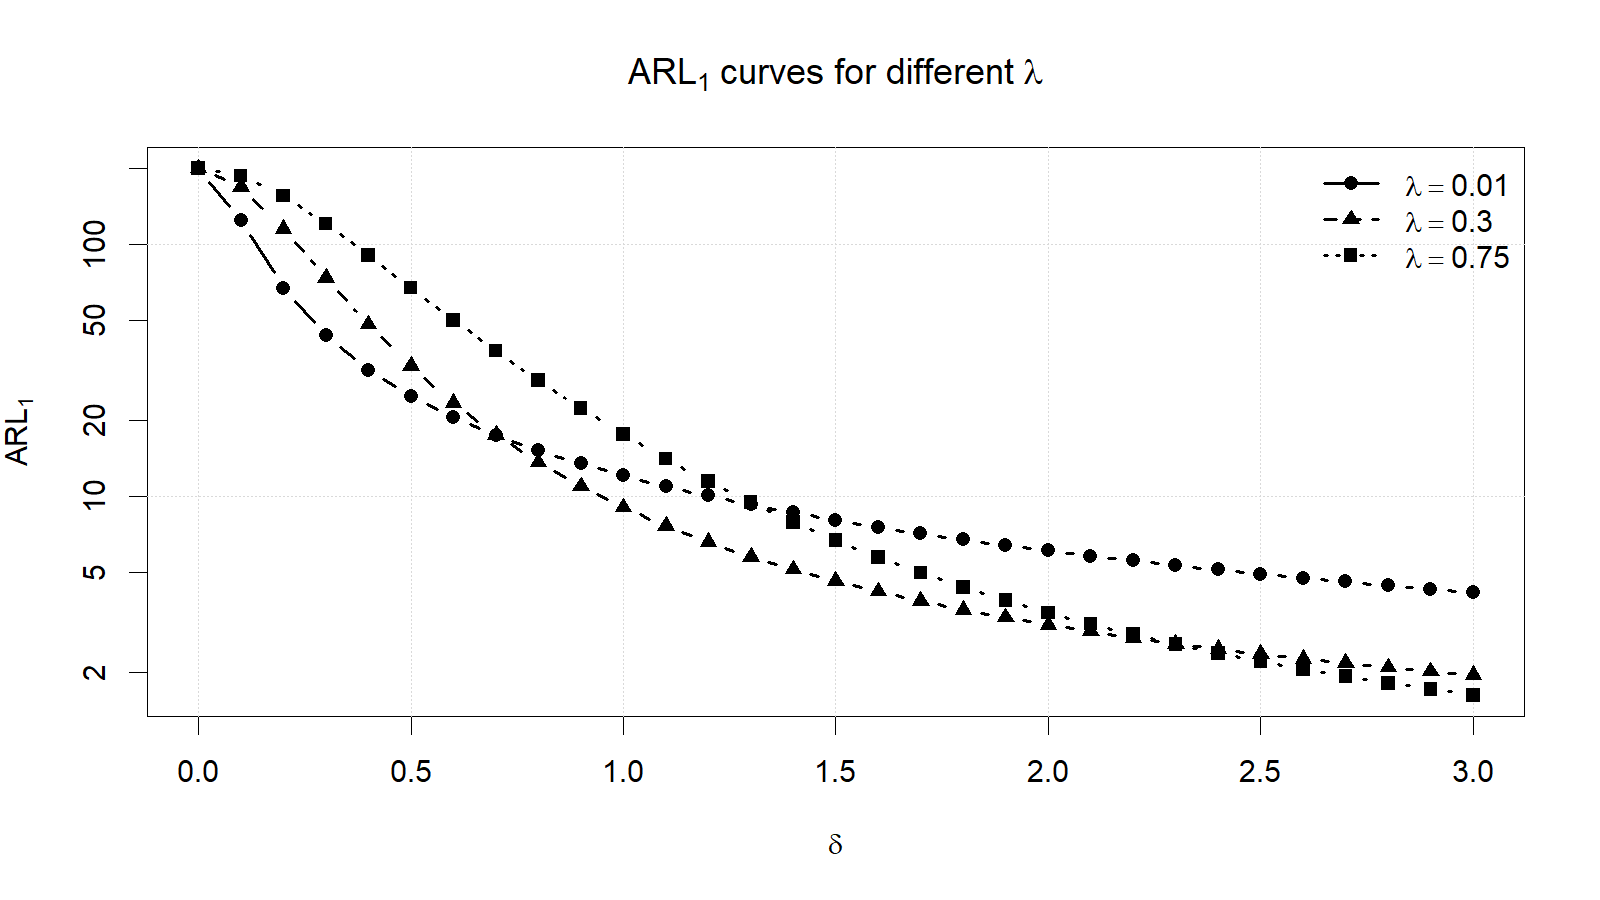
\includegraphics[width=1\textwidth]{ch5_exercise_5_8_arl1_curves.png}
\end{figure}

From the plot, all three curves start from \(ARL_0=200\) when \(\delta=0\). As the shift size \(\delta\) increases, \(ARL_1\) decreases for all three values of \(\lambda\). This is reasonable because a larger mean shift is easier to detect.

For small shifts, such as \(\delta=0.1\), the chart with \(\lambda=0.01\) has the smallest \(ARL_1\). This indicates that a smaller \(\lambda\) is more effective for detecting small persistent shifts, because it gives stronger smoothing and has a longer memory.

For large shifts, such as \(\delta=3.0\), the chart with \(\lambda=0.75\) has the smallest \(ARL_1\). This indicates that a larger \(\lambda\) is more effective for detecting large shifts, because it gives more weight to the current observation and reacts more quickly.

Therefore, the choice of \(\lambda\) should depend on the size of the mean shift that we want to detect. A smaller \(\lambda\) is more suitable for detecting small and persistent shifts, because it gives more smoothing and uses more historical information. A larger \(\lambda\) is more suitable for detecting large shifts, because it gives more weight to new observations and reacts more quickly.

\section*{5.20}
\textbf{Sol.}

\[
\begin{array}{c|c|c|c|c|c|c|c}
\text{Case} & \eta & \mu_1 & \mu_2 & h & \lambda & u & \text{First signal} \\ \hline
(i) & \eta_1 & 0.25 & 4 & 0.1471 & 0.0162 & 2.7459 & \text{NA}\\
(ii) & \eta_1 & 1.00 & 4 & 0.7874 & 0.1813 & 2.5752 & 19\\
(iii) & \eta_1 & 0.25 & 6 & 0.1515 & 0.0207 & 4.2537 & \text{NA}\\
(iv) & \eta_2 & 0.25 & 4 & 0.3542 & 0.0188 & 12.6145 & 19\\
(v) & \eta_2 & 1.00 & 4 & 0.7697 & 0.1359 & 10.6114 & 19\\
(vi) & \eta_2 & 0.25 & 6 & 0.1430 & 0.0168 & 48.7509 & \text{NA}
\end{array}
\]

\begin{figure}[H]
    \centering
    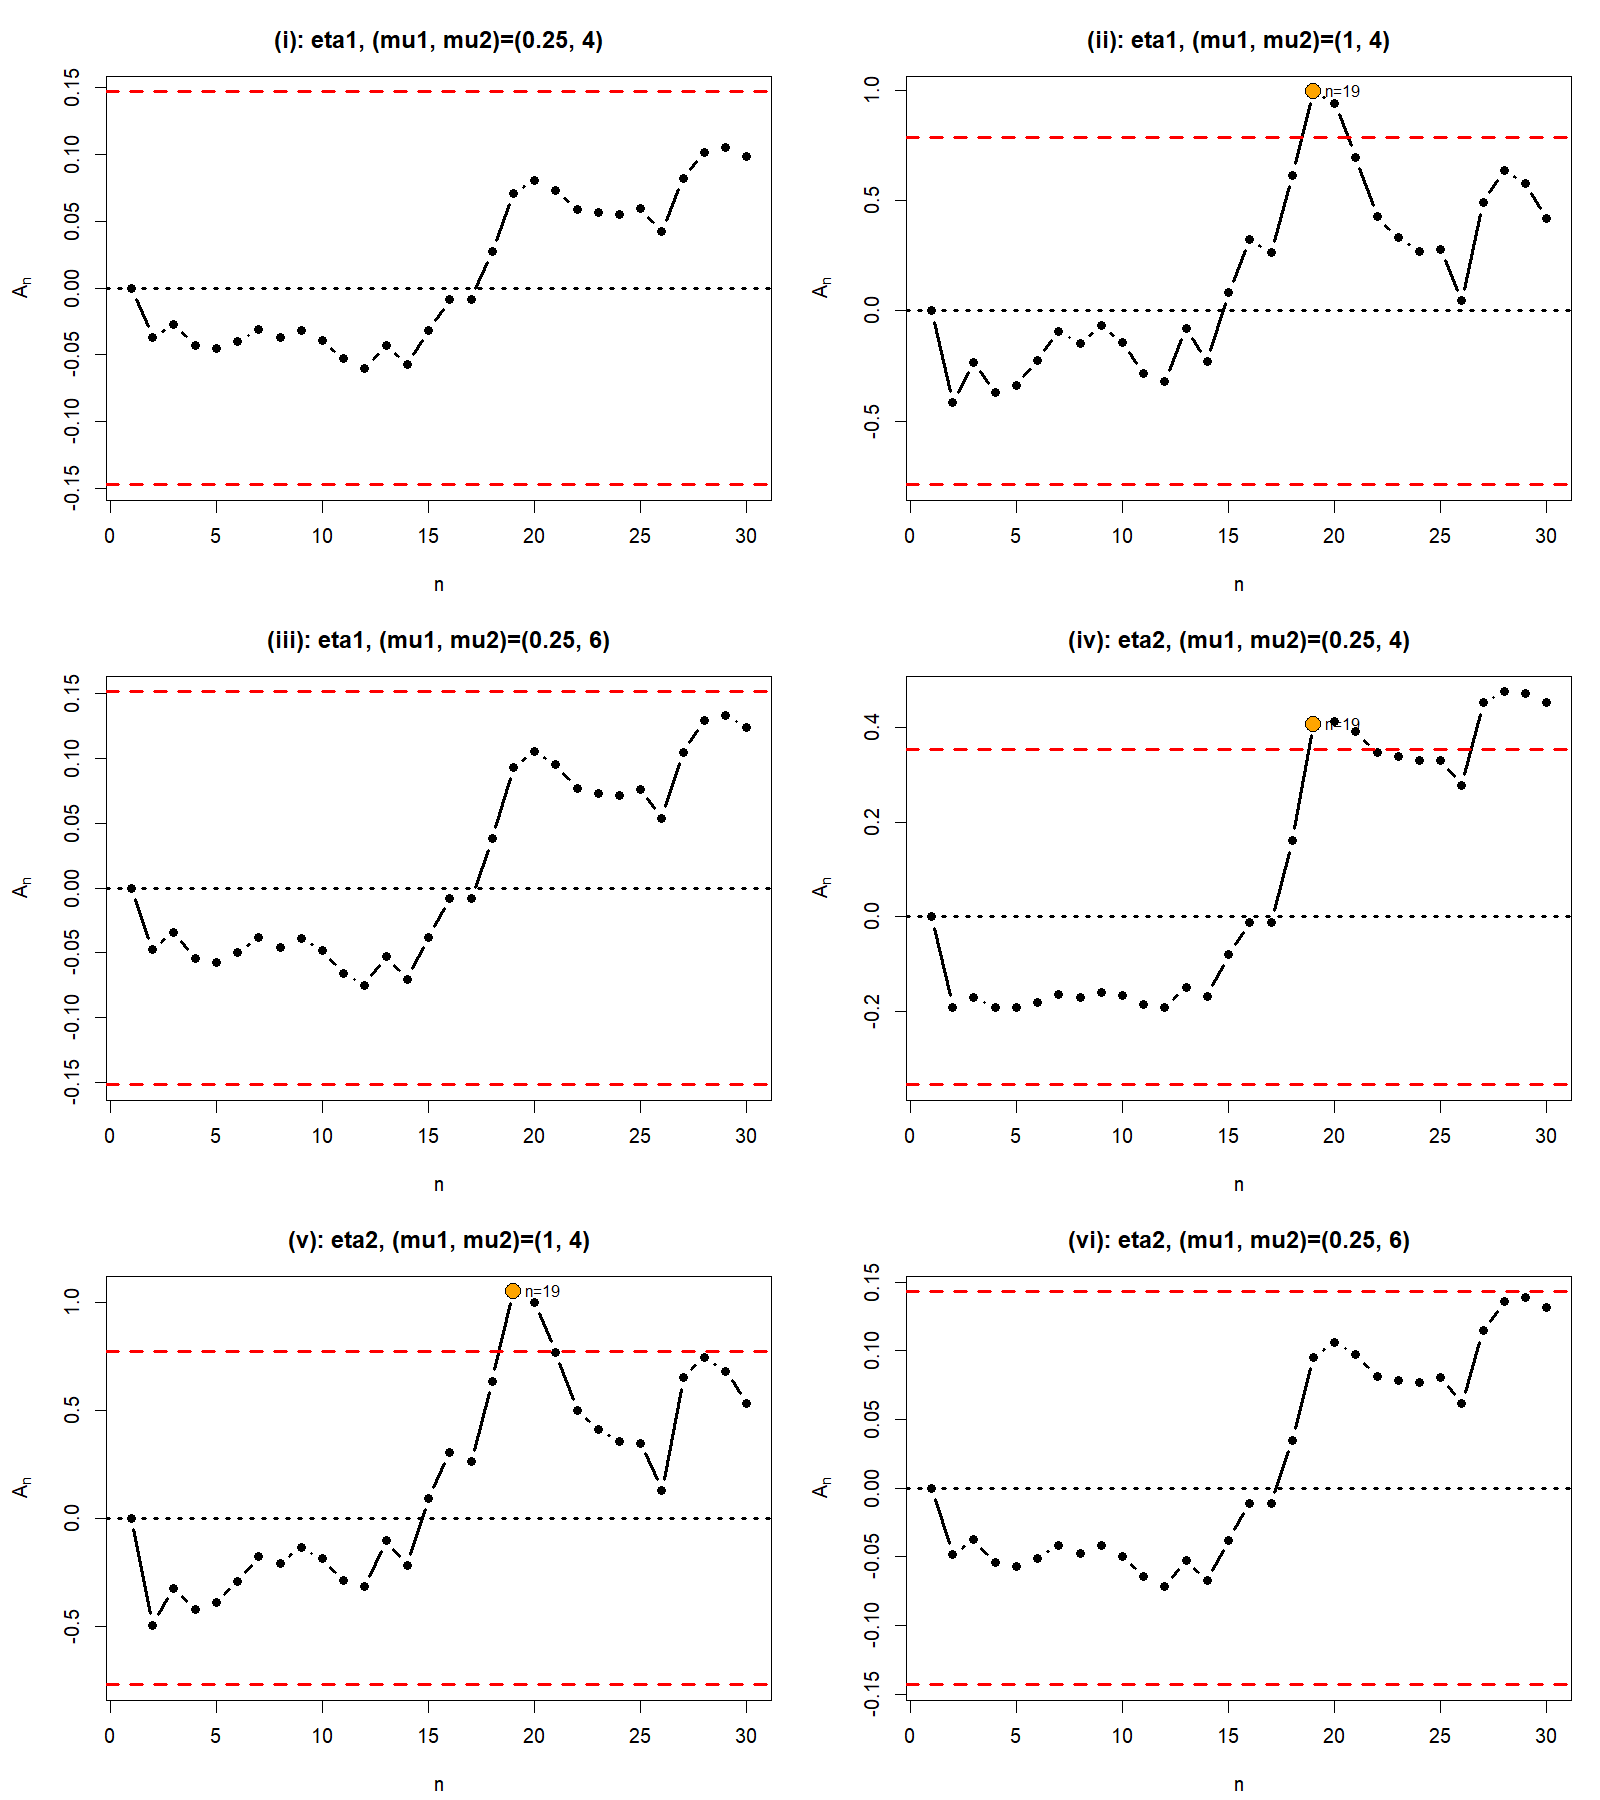
\includegraphics[width=1\textwidth]{ch5_exercise_5_20_AEWMA_3x2.png}
\end{figure}

From the results, cases (ii), (iv), and (v) give signals at \(n=19\), while cases (i), (iii), and (vi) do not give any signal within the first 30 observations.

This indicates that the detection result depends on the choice of the adaptive score function \(\eta(e_n)\) and the design parameters \((\mu_1,\mu_2)\). In this dataset, the observations around \(n=18\) and \(n=19\), especially \(X_{18}=2.2\) and \(X_{19}=2.7\), create a relatively large upward movement. Therefore, the more sensitive settings can detect this upward shift at \(n=19\).

For \(\eta_1\), case (ii) gives a signal, but cases (i) and (iii) do not. This is mainly because case (ii) has a larger \(\lambda\), so the adaptive EWMA statistic reacts more quickly to recent observations.

For \(\eta_2\), cases (iv) and (v) give signals, while case (vi) does not. This shows that different choices of \((\mu_1,\mu_2)\) and \(u\) can change the sensitivity of the chart. In particular, case (vi) has a very large \(u\), so the statistic changes more smoothly and does not cross the control limit in these 30 observations.

However, whether the chart can detect the shift depends on the choice of \(\eta(e_n)\) and the parameter settings.

\end{document}